\documentclass[aspectratio=169,11pt]{beamer}
\usepackage{amsmath,amssymb,mathtools,bm}
\usepackage{xeCJK}
\usepackage{pgfplots}
\pgfplotsset{compat=1.18}
\setCJKmainfont{Noto Sans CJK SC}
\setCJKsansfont{Noto Sans CJK SC}
\usetheme{Boadilla}
\usecolortheme{dolphin}
\setbeamertemplate{navigation symbols}{}
\setbeamertemplate{footline}[frame number]
\newcommand{\dd}{\mathrm d}
\newcommand{\ii}{\mathrm i}
\newcommand{\id}{\mathbb I}
\newcommand{\ket}[1]{\lvert #1\rangle}
\title{第 0 讲：散射理论序言}
\subtitle{散射计算中的分解、求逆与物理条件}
\author{Baiting Tian}
\date{}
\begin{document}

\begin{frame}
\titlepage
\end{frame}

\begin{frame}{含时演化：散射过程的物理图像}
\[
H=H_0+V,\qquad
\ket{\Psi(t)}=e^{-\ii H(t-t_0)/\hbar}\ket{\Psi(t_0)}.
\]
\begin{itemize}
\item 准备一个入射波包，观察它进入相互作用区域。
\item 波包与靶发生相互作用，随后向不同方向或通道传播。
\item 远处的探测器记录出射粒子的分布。
\end{itemize}
后面要把这个过程转成可计算的方程，并保留正确的入射、出射条件。
\end{frame}

\begin{frame}{时间与空间的乘积结构}
用时间函数和空间函数的乘积及其叠加组织时空依赖：
\[
\Psi(t,\bm r)=\sum_a T_a(t)\psi_a(\bm r),
\qquad \mathcal F_t\otimes\mathcal H_{\bm r}.
\]
当 $H$ 不显含时间时，方程中的算子分别作用于两个因子：
\[
\mathcal D=\ii\hbar\partial_t\otimes\id-\id\otimes H.
\]
后面选择能量、角度和通道基底时，都要先组织展开，再检查算子是否让各模式解耦。
\medskip

$\mathcal F_t$ 表示时间函数空间。时间仍是演化参数，连续标签的求和用积分代替。
% [EN] Time modes organize spacetime functions, not an extra quantum subsystem / [CN] 时间模态组织时空函数，并不引入额外的量子子系统。
\note{乘积函数空间的数学背景：\url{https://www.ime.usp.br/~tausk/texts/TensorL2.pdf}}
\end{frame}

\begin{frame}{谐波模态与定能问题}
指数函数是时间微分算子的广义本征函数：
\[
\partial_t e^{\pm\ii\omega t}=\pm\ii\omega e^{\pm\ii\omega t}.
\]
取 $e^{-\ii\omega t}$ 约定，$\ii\hbar\partial_t$ 在该模式上作用等价于乘 $E=\hbar\omega$：
\[
\Psi_E(t,\bm r)=e^{-\ii Et/\hbar}\psi_E(\bm r),
\qquad H\psi_E=E\psi_E.
\]
\begin{itemize}
\item $H$ 不显含时间时，不同能量模式可以分别求解。
\item 一般波包是这些模式的叠加，叠加系数由初态决定。
\end{itemize}
后面固定入射能量计算振幅和截面，就以这种定能分解为起点。
\note{定态分离与波包叠加：\url{https://www.damtp.cam.ac.uk/user/tong/qm/qmhtml/S2.html}}
\end{frame}

\begin{frame}{受迫振动与后续散射计算}
用一个熟悉的初值问题，预演后面会遇到的计算困难。取单位质量：
\[
\ddot x+\omega_0^2x=f(t),\qquad x(0)=x_0,\quad\dot x(0)=v_0.
\]
贯穿本讲的具体例子是
\[
f(t)=F_0\cos\Omega t\quad(t\ge0),\qquad
x_0=v_0=0,\qquad 0<\Omega\ne\omega_0.
\]
\begin{itemize}
\item 未知解也出现在源项中时，怎样构造积分方程并逐次修正？
\item 换表象以后，哪些算子简化了，哪些耦合与物理条件仍要处理？
\end{itemize}
这些问题会在后续的 LS 方程、分波与通道耦合、散射边界条件中反复出现。
\end{frame}

\begin{frame}{Picard：未知解怎样进入积分方程？}
后面会遇到未知解出现在方程两侧的积分方程。先把振子方程积分两次：
\[
x(t)=x_0+v_0t+\int_0^t(t-\tau)
\bigl[f(\tau)-\omega_0^2x(\tau)\bigr]\dd\tau.
\]
用上一轮的轨迹生成下一轮：
\[
x^{(n+1)}(t)=x_0+v_0t+\int_0^t(t-\tau)
\bigl[f(\tau)-\omega_0^2x^{(n)}(\tau)\bigr]\dd\tau.
\]
\begin{itemize}
\item 每轮用上一次的 $x$ 计算回复力，再更新整条轨迹。
\item 后面的 LS 方程与 Born 迭代也用近似解生成新的源，再修正近似解。
\end{itemize}
逐次修正的思想可以沿用；散射迭代的收敛性需要结合势与能量判断。
\end{frame}

\begin{frame}{Runge--Kutta：一阶系统的数值推进}
后面的径向方程通常没有解析解，需要从原点附近沿 $r$ 向外积分。
\[
\bm y=\begin{pmatrix}x\\v\end{pmatrix},\qquad
\dot{\bm y}=\bm F(t,\bm y)
=\begin{pmatrix}v\\f(t)-\omega_0^2x\end{pmatrix}.
\]
用已知的位置与速度，在一个小区间内估计运动。
RK4 组合当前步内四次评估的斜率 $\bm k_1,\ldots,\bm k_4$：
\[
\bm y_{n+1}=\bm y_n+\frac h6
(\bm k_1+2\bm k_2+2\bm k_3+\bm k_4).
\]
\begin{itemize}
\item 这里沿时间推进；后面沿半径推进，获得正则径向解。
\item 还要在远场匹配入射、出射波才能读取相移，并检查步长收敛。
\end{itemize}
\end{frame}

\begin{frame}{Numerov：二阶方程的三点递推}
后面的径向方程同样不含一阶导数，可以直接利用二阶结构。振子中令
\[
t_n=nh,\qquad a=\frac{h^2\omega_0^2}{12},\qquad f_n=f(t_n).
\]
Numerov 格式直接联系三个相邻时刻：
\[
\begin{aligned}
(1+a)x_{n+1}={}&2(1-5a)x_n-(1+a)x_{n-1}\\
&+\frac{h^2}{12}\bigl(f_{n+1}+10f_n+f_{n-1}\bigr).
\end{aligned}
\]
\begin{itemize}
\item 振子由初值及 Taylor 展开启动两个点，再逐步递推。
\item 径向问题的有效系数随 $r$ 变化，需要使用相应的变系数格式。
\end{itemize}
后面选择数值格式时要利用方程结构，并分别处理原点启动与远场匹配。
\end{frame}

\begin{frame}{Fourier：哪些算子会被简化？}
后面在动量表象中，自由动能变成乘法，相互作用仍可耦合不同动量。
\[
x(t)=\int\frac{\dd\omega}{2\pi}e^{-\ii\omega t}\widetilde x(\omega),
\qquad \partial_t^2 e^{-\ii\omega t}=-\omega^2e^{-\ii\omega t}.
\]
在每个频率上，微分方程化为代数关系：
\[
(\omega_0^2-\omega^2)\widetilde x=\widetilde f,
\qquad
\widetilde x(\omega)=\frac{\widetilde f(\omega)}{\omega_0^2-\omega^2}
\quad(\omega\ne\pm\omega_0).
\]
\begin{itemize}
\item 振子的时间系数恒定，不同频率独立；极点处仍需选定响应。
\item 本例按 $f(t)=\theta(t)F_0\cos\Omega t$ 接通外力，取 $t<0$ 静止。
\end{itemize}
全时轴谐波按广义变换理解。后面换表象时，也要检查剩余耦合与物理条件。
\end{frame}

\begin{frame}{Laplace：变换以后初态在哪里？}
后面联系含时演化与能量域方程时，需要追踪初态怎样进入变换。
\[
X(s)=\int_0^\infty e^{-st}x(t)\dd t,\qquad
\mathcal L[\ddot x]=s^2X-sx_0-v_0.
\]
记 $F(s)=\mathcal L[f](s)$，则
\[
X(s)=\frac{F(s)+sx_0+v_0}{s^2+\omega_0^2}.
\]
\begin{itemize}
\item 振子的初值明确进入分子，变换后的方程仍携带这些已知数据。
\item 后面把时间传播写成能量域的 Green 算符时，也要保留初态并规定收敛方式。
\end{itemize}
变换把微分化为代数运算；初始数据和响应条件仍是求解的一部分。
\end{frame}

\begin{frame}{Green 函数：单位脉冲的响应}
后面需要知道一处源怎样影响别处的波函数。先看单位脉冲怎样驱动振子：
\[
(\partial_t^2+\omega_0^2)G_R(t)=\delta(t),
\qquad G_R(t<0)=0.
\]
单位冲量令速度跃变 $1$，随后系统自由振动：
\[
G_R(0^+)=0,\qquad \dot G_R(0^+)=1,
\]
\[
G_R(t)=\theta(t)\frac{\sin\omega_0t}{\omega_0}.
\]
下标 $R$ 表示推迟响应。后面的自由 Green 算符也先解决给定源的响应问题。
\end{frame}

\begin{frame}{Green 函数：已知外源与未知源}
后面的散射源 $V\psi$ 含有未知波函数。先理解已知外力怎样产生响应：
\[
x(t)=x_h(t)+\int_0^tG_R(t-\tau)f(\tau)\dd\tau,
\]
\[
x_h(t)=x_0\cos\omega_0t+\frac{v_0}{\omega_0}\sin\omega_0t.
\]
\begin{itemize}
\item $x_h$ 携带初值，卷积项叠加各时刻外力产生的响应。
\item 这里 $f$ 已知；散射中的 $V\psi$ 还依赖待求的 $\psi$。
\end{itemize}
因此，后面的响应关系本身成为积分方程，需要继续迭代或离散为线性方程组。
\note{Green 函数与初值项：\url{https://tonic.physics.sunysb.edu/~dteaney/F16_Phy505/lectures/green.pdf}}
\end{frame}

\begin{frame}{因果响应的频域 Green 函数}
后面 Green 算符的分母可能为零，需要规定怎样求逆。振子先用 $\epsilon>0$ 保证收敛：
\[
\widetilde G_R(\omega)
=\lim_{\epsilon\downarrow0}\int_0^\infty
 e^{\ii\omega\tau-\epsilon\tau}
 \frac{\sin\omega_0\tau}{\omega_0}\dd\tau
=\frac{1}{\omega_0^2-(\omega+\ii0^+)^2}.
\]
若系统在 $t<0$ 静止，则
\[
\widetilde x(\omega)=\widetilde G_R(\omega)\widetilde f(\omega).
\]
\begin{itemize}
\item 时间域的响应条件，在频域中指定了极点的位置。
\item 后面的 $(E-H_0+\ii0^+)^{-1}$ 也需要附带物理条件来定义。
\end{itemize}
分母为零时，物理条件参与逆算符的定义。
\end{frame}

\begin{frame}{极点绕行与因果条件}
后面 $+\ii0^+$ 为什么对应出射波？先看绕行规定怎样选出振子的响应。
\[
G_R(\tau)=\int_{-\infty}^{\infty}\frac{\dd\omega}{2\pi}
\frac{e^{-\ii\omega\tau}}{\omega_0^2-(\omega+\ii0^+)^2}.
\]
极点位于 $\omega=\pm\omega_0-\ii0^+$，都在实轴下方。
\begin{itemize}
\item $\tau>0$：指数在下半平面衰减，向下闭合并拾取留数。
\item $\tau<0$：向上闭合，内部没有极点，因此响应为零。
\end{itemize}
\[
G_R(\tau)=\theta(\tau)\frac{\sin\omega_0\tau}{\omega_0}.
\]
振子选择时间上的因果响应；散射选择空间上的出射行为，各自通过极点规定表达。
\end{frame}

\begin{frame}{可解模型与数值结果的检查}
用本例的精确解，检查不同算法是否满足同一个方程与零初值：
\[
x(t)=\frac{F_0}{\omega_0^2-\Omega^2}
\bigl(\cos\Omega t-\cos\omega_0t\bigr),\qquad t\ge0.
\]
\begin{center}
% [EN] Plot the dimensionless exact response so the frequency ratio fixes the curve / [CN] 绘制无量纲精确响应，使曲线只取决于两个频率的比值。
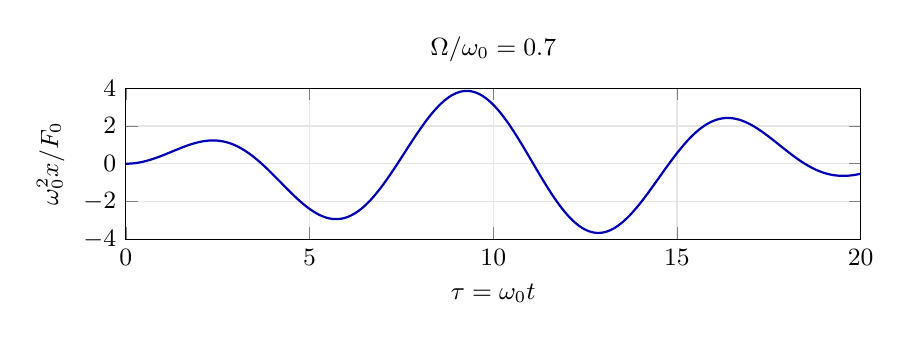
\begin{tikzpicture}
\begin{axis}[
width=0.9\textwidth,height=3.5cm,
xmin=0,xmax=20,ymin=-4,ymax=4,
xlabel={$\tau=\omega_0t$},ylabel={$\omega_0^2x/F_0$},
xtick={0,5,10,15,20},ytick={-4,-2,0,2,4},
grid=major,grid style={gray!20},
tick label style={font=\small},label style={font=\small},
title={$\Omega/\omega_0=0.7$},title style={font=\small},
]
\addplot[blue!70!black,thick,domain=0:20,samples=301]
{(cos(deg(0.7*x))-cos(deg(x)))/(1-0.7^2)};
\end{axis}
\end{tikzpicture}
\end{center}
后面同样用可解势与步长、网格收敛，检查散射数值解的精度。
\end{frame}

\begin{frame}{耦合振子与散射中的通道耦合}
散射中分离能量或角度后，还可能剩下一组耦合方程。振子中取正定的 $K$：
\[
\ddot{\bm x}+K\bm x=\bm f(t),\qquad
K=\begin{pmatrix}\omega_1^2&\lambda\\\lambda&\omega_2^2\end{pmatrix}.
\]
时间函数与振子分量构成 $\mathcal F_t\otimes\mathbb C^2$，推迟响应为
\[
\widetilde{\bm x}(\omega)
=\bigl[K-(\omega+\ii0^+)^2I\bigr]^{-1}\widetilde{\bm f}(\omega).
\]
\begin{itemize}
\item 对角化 $K$ 可以得到简正模；在原来的分量基底中仍有耦合。
\item 散射通道有类似的矩阵结构，连续的动量标签则对应积分核。
\end{itemize}
后面选定表象之后，还要用矩阵求解或积分方程方法处理剩余耦合。
\end{frame}

\begin{frame}{定能与分波：散射问题的变量组织}
在散射中，先分离时间模态，再用径向和角向函数组织空间：
\[
\Psi_E(t,\bm r)=e^{-\ii Et/\hbar}\psi_E(\bm r),
\]
\[
L^2(\mathbb R^3,\dd^3r)
\simeq L^2(\mathbb R_+,r^2\dd r)\otimes L^2(S^2,\dd\Omega),
\]
\[
\psi_E(\bm r)=\sum_{lm}\frac{u_{Elm}(r)}{r}Y_{lm}(\hat{\bm r}).
\]
\begin{itemize}
\item 定能模式组织时间依赖，球谐函数组织角度依赖。
\item 改用 $u=rR$ 后，径向内积的测度变成 $\dd r$。
\end{itemize}
能否独立求解各分波，接下来要看 Hamiltonian 的结构。
\end{frame}

\begin{frame}{中心势中的算子分离与通道耦合}
对无自旋中心势，改用约化径向函数 $u=rR$ 后，
\[
H=h_r\otimes\id+\frac{1}{2\mu r^2}\otimes\bm L^2,
\qquad
h_r=-\frac{\hbar^2}{2\mu}\frac{\dd^2}{\dd r^2}+V(r).
\]
球谐函数使角动量算子对角化：
\[
\bm L^2Y_{lm}=\hbar^2l(l+1)Y_{lm}.
\]
\begin{itemize}
\item 每个 $l,m$ 对应一个独立的径向问题，其中保留离心项。
\item 更一般的势可耦合不同分波，得到一组耦合的径向方程。
\end{itemize}
乘积展开始终提供组织方式，解耦则来自相应的算子结构与对称性。
% [EN] The radial-angular operator is written after the unitary reduction u=rR / [CN] 径向与角向算子的表达式使用了 u=rR 的幺正约化。
\note{中心势与分波：\url{https://farside.ph.utexas.edu/teaching/qm/Quantumhtml/node86.html}}
\end{frame}

\begin{frame}{径向积分与远场匹配}
取 $E=\hbar^2k^2/(2\mu)>0$，短程实中心势下的分波满足
\[
u_l''(r)+\left[k^2-\frac{l(l+1)}{r^2}
-\frac{2\mu V(r)}{\hbar^2}\right]u_l(r)=0.
\]
\begin{itemize}
\item 对原点正则的势，由 $u_l(r)\propto r^{l+1}$ 启动积分。
\item 用 Numerov 或 Runge--Kutta 沿 $r$ 推进。
\item 在远处匹配自由解，提取相移：
\end{itemize}
\[
u_l(r)\sim A_l\sin\bigl(kr-l\pi/2+\delta_l\bigr).
\]
振子的初值规定怎样开始运动；散射的空间条件规定正则性与入射、出射行为。
\end{frame}

\begin{frame}{Green 算符与散射边界条件}
把相互作用看成依赖未知波函数的源：
\[
(E-H_0)\ket{\psi}=V\ket{\psi}.
\]
给定同能量的自由入射态 $\ket{\phi}$，选择出射 Green 算符后得到
\[
G_0^{(+)}(E)=(E-H_0+\ii0^+)^{-1},\qquad
\ket{\psi^{(+)}}=\ket{\phi}+G_0^{(+)}V\ket{\psi^{(+)}}.
\]
\begin{itemize}
\item 振子的推迟 Green 函数规定时间上的因果响应。
\item 散射中的 $+\ii0^+$ 规定源产生空间上的出射波：
\end{itemize}
\[
\psi^{(+)}(\bm r)\sim e^{\ii kz}+f(\hat{\bm r})\frac{e^{\ii kr}}{r}.
\]
物理条件随问题改变，带条件求逆的思想继续沿用。
\end{frame}

\begin{frame}{进入散射计算时会遇到的问题}
\renewcommand{\arraystretch}{1.45}
\begin{tabular}{@{}p{0.43\textwidth}p{0.53\textwidth}@{}}
\textbf{后面会遇到的问题}&\textbf{振子中已经见过的处理思路}\\\hline
定能、分波以后，是否还会耦合？&先选乘积基，再检查算子与剩余矩阵\\
未知解也出现在源项中，怎样求解？&积分方程的逐次修正，并检查收敛\\
没有解析解，怎样计算径向波函数？&Runge--Kutta、Numerov 推进，再作远场匹配\\
分母为零时，怎样定义带条件的逆？&Green 函数配合极点规定与物理条件\\
剩余的通道或动量耦合怎样处理？&矩阵求解，或积分方程的离散与迭代
\end{tabular}
\medskip

后续从自由态、渐近态和 $S$ 矩阵开始，把这些方法用于具体的散射问题。
\end{frame}

\end{document}
